\subsection{拉伸构建杯零件三维模型}
完成杯零件的主视图绘后就可以用拉伸法构建杯零件的三维模型,不需要对圆进行面域操作。
\begin{procedure}
\item 将大圆拉伸为圆柱。

启动【拉伸】命令的方法有:
\begin{itemize}
\item 键盘输入EXTRUDE\index{extrude}或EXT
\item 【绘图】$\rightarrow$【建模】$\rightarrow$【拉伸】。
\item 【建模】$\triangleright$【拉伸】图标
\includegraphics[scale=0.7]{extrudetool.png}。
\end{itemize}
首先以图\ref{fig:extrudeselecta}所示的方式选择大圆进行拉伸,选中大圆后,该圆会以虚线方式表示。
\begin{figure}[htbp]
\centering
\subfloat[]{\label{fig:extrudeselecta}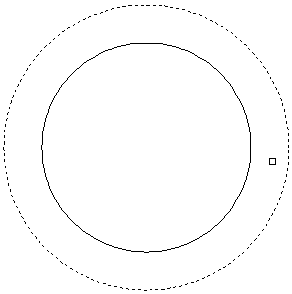
\includegraphics[scale=0.8]{extrudeselect.png}}\hspace{20pt}
\subfloat[]{\label{fig:extrudeselectb}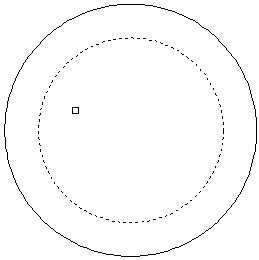
\includegraphics[scale=0.9]{extrudeselect1.png}}
\caption{拉伸过程}
\end{figure}
\begin{lstlisting}
|命令: EXTRUDE|
|当前线框密度:  ISOLINES=4,闭合轮廓创建模式 = 实体|
|选择要拉伸的对象或 [模式(MO)]: 找到 1 个|
|选择要拉伸的对象或 [模式(MO)]:|
\end{lstlisting}
接下来输入拉伸高度。做拉伸操作时,拉伸高度的值既可以取正值,也可以取负值,两者的区别是拉伸的方向的不同。拉伸高度取正值是沿$Z$轴正方向进行拉伸,取负值则是沿$z$轴负方向拉伸。本例的拉伸方向是由前向后拉伸,即要沿$z$轴的负方向进行拉伸,因此取负值。
\begin{lstlisting}
|指定拉伸的高度或 [方向(D)/路径(P)/倾斜角(T)/表达式(E)]: -15|
\end{lstlisting}
\item 将小圆拉伸为圆柱。按图\ref{fig:extrudeselectb}所示的方式,用拾取状态的鼠标选取小圆做为拉伸对象,若再次选择大圆将不能够选中,因为此时的大圆已经是一个实体。
\begin{lstlisting}
|命令: EXTRUDE|
|当前线框密度:  ISOLINES=4,闭合轮廓创建模式 = 实体|
|选择要拉伸的对象或 [模式(MO)]: 找到 1 个|
|选择要拉伸的对象或 [模式(MO)]:|
|指定拉伸的高度或 [方向(D)/路径(P)/倾斜角(T)/|
|表达式(E)] $<-15.0000>$: -10|
\end{lstlisting}

\item 将视图切换为【西南等轴测】。
\item 从大圆柱中减去小圆柱。
按照图\ref{fig:subtractselect1}所示的方式选择大圆柱作为被减实体。
\begin{lstlisting}
|命令: SUBTRACT |
|选择要从中减去的实体、曲面和面域...|
|选择对象: 找到 1 个|
\end{lstlisting}
按照图\ref{fig:subtractselect2}所示的方式选择小圆柱作为要减去的实体。
\begin{lstlisting}
|选择对象:  选择要减去的实体、曲面和面域...|
|选择对象: 找到 1 个|
|选择对象:|
\end{lstlisting}
\begin{figure}[htbp]
\centering
\subfloat[]{\label{fig:subtractselect1}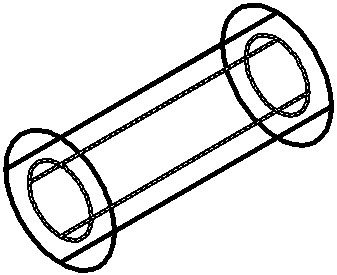
\includegraphics[scale=0.7]{subtractselect1.png}}\hspace{20pt}
\subfloat[]{\label{fig:subtractselect2}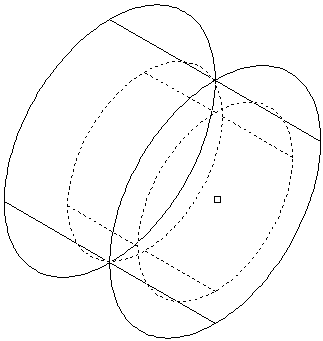
\includegraphics[scale=0.7]{subtractselect2.png}}
\caption{差集过程}
\end{figure}
\item 切换视觉样式为灰度。点击【视图】菜单中【视觉样式】子菜单中的【灰度】项。
\end{procedure}

通过上述步骤,我们获得了与图\ref{fig:beimodel}一样的三维模型。

拉伸命令的注意事项和技巧:
\begin{tips}
\item 拉伸命令不仅可以用于矩形、圆、多边形,也可以用于异形面域对象。
\item 用圆、矩形、正多边形做拉伸对象,不需要先进行面域操作。
\item 若拉伸的对象不是圆、矩形、正多边形或面域对象,拉伸后将是空间平面,而非实体。
\end{tips}
\endinput